\documentclass{beamer}

\usetheme{Singapore}
\usepackage{german}
\usepackage[utf8x]{inputenc}
\usepackage{listings}
\lstset{language=Java, frame=tlrb, keywordstyle=\color{red}, breaklines=true,  basicstyle=\footnotesize}


\begin{document}
\title{Graphicus}   
\author{Paul Stahr und Yakup Ates} 
\date{\today}
%\logo{\includegraphics[scale=0.14]{ BILD }}

\begin{frame}
\titlepage
\end{frame}

\begin{frame}[allowframebreaks]
\frametitle{Inhaltsverzeichnis}\tableofcontents
\end{frame}
%%%%%%%%%%%%%%%%%%%%%%%%%%%%%%%%%%%%%%%%%%%%%%%%%%%%%%%%%%%%%%%%%%%%%%%%%%%%%%%%%%
\section{Systemanforderungen}
\begin{frame}\frametitle{Systemanforderungen}
 \begin{itemize}
  \item OpenGL 
  \item Java (mind. V. 6)
  \item LWJGL (mind. V. 1.7.2)
  \item 1GHZ CPU, 512MB RAM, 128MB VRAM
 \end{itemize}
\end{frame}

%%%%%%%%%%%%%%%%%%%%%%%%%%%%%%%%%%%%%%%%%%%%%%%%%%%%%%%%%%%%%%%%%%%%%%%%%%%%%%%%%%
\section{Algorithmen}

  \begin{frame}[shrink]
    \frametitle{Übersicht}
    \tableofcontents[currentsection]
  \end{frame}
%%%%%%%%%%%%%%%%%%%%%%%%%%%%%%%%%%%%%%%%%%%%%%%%%%%%%%%%%%%%%%%%%%%%%%%%%%%%%%%%%%

\subsection{Wurzel} 
\begin{frame}\frametitle{Wurzel - Mathematische Ebene} 
Newtonsches N\"aherungsverfahren: ($ \sqrt a $)
\begin{itemize}
 \item $ f(x) = x^2 - a $
\end{itemize}

Nullstellenbestimmung mit Iterationsformel:
\begin{itemize}
 \item $ x_{n+1} = x_n - \frac{x^2_n - a}{2 \cdot x_n} $
\end{itemize}

 Daraus resultiert:
\begin{itemize}
 \item $ x_{n+1} = \frac{ x^2_n + a}{2 \cdot x_n } \qquad $
\end{itemize}
\end{frame}
%%%%%%%%%%%%%%%%%%%%%%%%%%%%%%%%%%%%%%%%%%%%%%%%%%%%%%%%%%%%%%%%%%%%%%%%%%%%%%%%%%

\begin{frame}[fragile]{Wurzel - Informatik Ebene}
	\begin{exampleblock}{Algorithmus}
		\begin{lstlisting}
public static final double sqrt(final double n){
  if(n<0)
    return Double.NaN;
  if(n==0)
    return 0;
  double erg=n;
  for(int i=1;i!=11;i++)
    erg=(erg*erg+n)/(2*erg);
  return erg;        
}
		\end{lstlisting}
	\end{exampleblock}
\end{frame}
%%%%%%%%%%%%%%%%%%%%%%%%%%%%%%%%%%%%%%%%%%%%%%%%%%%%%%%%%%%%%%%%%%%%%%%%%%%%%%%%%%

\subsection{Gr\"o\ss{}ter gemeinsamer Teiler}
\begin{frame}\frametitle{ggT - Mathematische Ebene} 
Euklids-Algorithmus\newline
\begin{tabular}[b]{|l|l|l|}
\hline
n & \(r_n\) & Variable\\
\hline\hline
0 & 9 & a\\
\hline
1 & 5 & b\\
\hline
2 & 4 & a\\
\hline
3 & 1 & b\\
\hline
3 & 0 & a\\
\hline
\end{tabular}
\end{frame}
%%%%%%%%%%%%%%%%%%%%%%%%%%%%%%%%%%%%%%%%%%%%%%%%%%%%%%%%%%%%%%%%%%%%%%%%%%%%%%%%%%

\begin{frame}[fragile]{ggT - Informatik Ebene}
	\begin{exampleblock}{Algorithmus}
		\begin{lstlisting}
public static final long ggt (long a, long b){
  if (a < 0)
    a = -a;
  if (b < 0)
    b = -b;
  while ((a%=b)!=0)
    if ((b%=a)==0)
      return a;
  return b;
}
		\end{lstlisting}
	\end{exampleblock}
\end{frame}
%%%%%%%%%%%%%%%%%%%%%%%%%%%%%%%%%%%%%%%%%%%%%%%%%%%%%%%%%%%%%%%%%%%%%%%%%%%%%%%%%%
\subsection{Kleinstes gemeinsames Vielfaches} 
\begin{frame}\frametitle{kgv - Mathematische Ebene} 
\(kgv(a,b) = \frac{a \cdot b}{ggt(a,b)} = \frac{a}{ggt(a,b)} \cdot b\)\newline
(Auch bei Ganzzahlen m"oglich.)
\end{frame}
%%%%%%%%%%%%%%%%%%%%%%%%%%%%%%%%%%%%%%%%%%%%%%%%%%%%%%%%%%%%%%%%%%%%%%%%%%%%%%%%%%
\begin{frame}[fragile]{kgv - Informatik Ebene}
	\begin{exampleblock}{Funktion}
		\begin{lstlisting}
public static final long kgv (long a, long b){
  if (a < 0)
    a = -a;
  if (b < 0)
    b = -b;
  final long c = a / ggt(a,b);
  final long kgv = b * c;
  return kgv / b == c ? kgv : -1;
}
		\end{lstlisting}
	\end{exampleblock}
\end{frame}
%%%%%%%%%%%%%%%%%%%%%%%%%%%%%%%%%%%%%%%%%%%%%%%%%%%%%%%%%%%%%%%%%%%%%%%%%%%%%%%%%%
\subsection{Anzahl der Kombinationen} 
\begin{frame}\frametitle{Anzahl der Kombinationen - Mathematische Ebene} 
\({n \choose k} = ncr(n,k)=\frac{n!}{k! \cdot (n-k)!} = \prod \limits_{i=1}^{k} \frac{n-k+i}{i} \)\newline
\({n \choose k} = {n \choose n-k}\)
\end{frame}
%%%%%%%%%%%%%%%%%%%%%%%%%%%%%%%%%%%%%%%%%%%%%%%%%%%%%%%%%%%%%%%%%%%%%%%%%%%%%%%%%%
\begin{frame}[fragile]{Anzahl der Kombinationen - Informatik Ebene}
\begin{lstlisting}
public static final long ncr (final long n, long k){
  if (k < 0 || n < 0 || n < k)
    return -2;
  if (n < fakCacheLong.length)
    return fakCacheLong[(int)n]/(fakCacheLong[(int)k]*fakCacheLong[(int)(n-k)]);
  if (n<k/2)
    k = n-k;
  long erg = 1;
  final long nk = n-k;
  for (int i=1;i<=k;i++)
    if ((erg /= i) != (erg *= nk + i) / (nk + i))
      return -1;
  return erg;
}
\end{lstlisting}
\end{frame}
%%%%%%%%%%%%%%%%%%%%%%%%%%%%%%%%%%%%%%%%%%%%%%%%%%%%%%%%%%%%%%%%%%%%%%%%%%%%%%%%%%
\section{Datentypen}
  \begin{frame}[shrink]
    \frametitle{Übersicht}
    \tableofcontents[currentsection]
  \end{frame}
%%%%%%%%%%%%%%%%%%%%%%%%%%%%%%%%%%%%%%%%%%%%%%%%%%%%%%%%%%%%%%%%%%%%%%%%%%%%%%%%%%
\subsection{Ganzzahl}
\begin{frame}\frametitle{Ganzzahl}
 \begin{itemize}
 \item Beispiel: 4
\item Wertebereich: $-2^{63}$ bis $2^{63}-1$
\item Verhalten bei "Uberlauf: Umwandlung in Flie"skommazahl oder Ergebnis = -1
\item Konvertierungsfunktion: int(a)
 \end{itemize}
\end{frame}
%%%%%%%%%%%%%%%%%%%%%%%%%%%%%%%%%%%%%%%%%%%%%%%%%%%%%%%%%%%%%%%%%%%%%%%%%%%%%%%%%%
\subsection{Flie"skommazahl}
\begin{frame}
\frametitle{Flie"skommazahl}
 \begin{itemize}
 \item Beispiel: 4.5
\item Wertebereich: $-1.797^{308}$ bis $1.797^{308}$
\item Verhalten bei "Uberlauf: Ersetzung durch \(\infty\)
\item Konvertierungsfunktion: float(a)
 \end{itemize}
\end{frame}
%%%%%%%%%%%%%%%%%%%%%%%%%%%%%%%%%%%%%%%%%%%%%%%%%%%%%%%%%%%%%%%%%%%%%%%%%%%%%%%%%%
\subsection{Zeichen}
\begin{frame}
\frametitle{Zeichen}
 \begin{itemize}
 \item Beispiel: '4'
\item Verhalten bei Berechnungen: Unicode-Wert wird zur Berechnung verwendet
\item Konvertierungsfunktion: char(a)
 \end{itemize}
\end{frame}
%%%%%%%%%%%%%%%%%%%%%%%%%%%%%%%%%%%%%%%%%%%%%%%%%%%%%%%%%%%%%%%%%%%%%%%%%%%%%%%%%%
\subsection{Zeichenkette}
\begin{frame}
\frametitle{Zeichenkette}
 \begin{itemize}
 \item Beispiel: \grqq Vier\grqq
\item Konvertierungsfunktion: string(a)
 \end{itemize}
\end{frame}
%%%%%%%%%%%%%%%%%%%%%%%%%%%%%%%%%%%%%%%%%%%%%%%%%%%%%%%%%%%%%%%%%%%%%%%%%%%%%%%%%%
\subsection{Liste}
\begin{frame}
\frametitle{Liste}
 \begin{itemize}
 \item Beispiel: \{4,4.5,'4',\grqq Vier\grqq\}
\item Zugriff: \{1,2,3\}[1] = 2
 \end{itemize}
\end{frame}
%%%%%%%%%%%%%%%%%%%%%%%%%%%%%%%%%%%%%%%%%%%%%%%%%%%%%%%%%%%%%%%%%%%%%%%%%%%%%%%%%%
\section{Funktionen}
  \begin{frame}[shrink]
    \frametitle{Übersicht}
    \tableofcontents[currentsection]
  \end{frame}
%%%%%%%%%%%%%%%%%%%%%%%%%%%%%%%%%%%%%%%%%%%%%%%%%%%%%%%%%%%%%%%%%%%%%%%%%%%%%%%%%%
\subsection{Aufrufe}
\begin{frame}\frametitle{Aufrufe}
 	  \begin{tabular}[b]{l|l}
	    Funktion					&	Aufruf	\\
	    \hline
	    Gr\"o\ss{}ter gemeinsamer Teiler		&	ggt(a,b)	\\
	    Kleinstes gemeinsames Vielfaches		&	kgv(a,b)	\\
	    Anzahl der Permutationen	        	&	npr(a,b)\\  
	    Anzahl der Kombinationen 			&	ncr(a,b) \\
	    Quadrat Wurzel				&	sqrt(a)	\\
	    Sinus					& 	sin(a) \\
	    Kosinus					&	cos(a)	\\
	    Tangens					&	tan(a)	\\
	    Logarithmus					&	log(a)	\\
	    Fakult\"at von a				&	a! \\
	    Addition					&	a + b \\
	    Subtraktion					&	a - b \\
	    Multiplikation				&	a * b \\	
	    \hline
	    \end{tabular}
\end{frame}
%%%%%%%%%%%%%%%%%%%%%%%%%%%%%%%%%%%%%%%%%%%%%%%%%%%%%%%%%%%%%%%%%%%%%%%%%%%%%%%%%%
\begin{frame}\frametitle{Aufrufe}
 	  \begin{tabular}[b]{l|l}
	    Funktion					&	Aufruf	\\
	    \hline
	    Division					&	a / b \\
	    Modulo					&	a \% b\\
	    Hyperbolischer Sinus			&	sinh(a)\\
	    Hyperbolischer Kosinus			& 	cosh(a)\\
	    Hyperbolischer Tangens			& 	tanh(a)\\
	    Variable definieren				&	define(a)\\
	    Variable l\"oschen				&	delete(a)\\
	    Aufl\"osen einer Gleichung			&	solve(m*x+b=0,b)\\
	    \hline
	    \end{tabular}
\end{frame}
%%%%%%%%%%%%%%%%%%%%%%%%%%%%%%%%%%%%%%%%%%%%%%%%%%%%%%%%%%%%%%%%%%%%%%%%%%%%%%%%%%
\subsection{Graphentypen}
\begin{frame}\frametitle{Graphentypen}
\begin{tabular}[b]{|l|l|}
\hline
2D Funktion & Ordnet jedem x einen y zu. \\
\hline
2D Parametrisch & Ordnet jedem t einen x und y zu \\
\hline
2D Polar & Bildet die Funktion in einem Kreis ab \\
\hline
2D Plot & Macht zwei Listen als Plot sichtbar \\
\hline
3D Linie & Ordnet jedem t ein x, y und z zu \\
\hline
3D Funktion & Ordnet jedem x und y ein z zu \\
\hline
3D Parametrisch & Ordnet jedem u und v ein x, y und z zu \\
\hline
3D Polar & noch nicht implementiert \\
\hline
3D Plot & Macht drei Listen als Plot sichtbar \\
\hline
Karthesisch & Graphen zb. der Art x*a+y*b+z*c=0 \\
\hline
\end{tabular}
\end{frame}
%%%%%%%%%%%%%%%%%%%%%%%%%%%%%%%%%%%%%%%%%%%%%%%%%%%%%%%%%%%%%%%%%%%%%%%%%%%%%%%%%%
\section{Programm/UI} 
  \begin{frame}[shrink]
    \frametitle{Übersicht}
    \tableofcontents[currentsection]
  \end{frame}
%%%%%%%%%%%%%%%%%%%%%%%%%%%%%%%%%%%%%%%%%%%%%%%%%%%%%%%%%%%%%%%%%%%%%%%%%%%%%%%%%%
\subsection{Hauptfenster} 
\begin{frame}\frametitle{Hauptfenster}
\includegraphics[height=0.7\textheight]{images/program/main-window.png}
\begin{itemize}
  \item Men\"uleiste und Toolmen\"u
  \item Anzeigefenster und Funktionen
\end{itemize}
\end{frame}
%%%%%%%%%%%%%%%%%%%%%%%%%%%%%%%%%%%%%%%%%%%%%%%%%%%%%%%%%%%%%%%%%%%%%%%%%%%%%%%%%%

\subsection{Zeichen} 
\begin{frame}\frametitle{Zeichen}
\centering
\includegraphics[width=0.6\textwidth]{images/program/characters-window.png}
\end{frame}
%%%%%%%%%%%%%%%%%%%%%%%%%%%%%%%%%%%%%%%%%%%%%%%%%%%%%%%%%%%%%%%%%%%%%%%%%%%%%%%%%%

\subsection{Optionen} 
\begin{frame}\frametitle{Option}
\includegraphics[width=0.5\textwidth]{images/program/settings0-window.png} 
\end{frame}

%%%%%%%%%%%%%%%%%%%%%%%%%%%%%%%%%%%%%%%%%%%%%%%%%%%%%%%%%%%%%%%%%%%%%%%%%%%%%%%%%%

\begin{frame}\frametitle{Option}
\includegraphics[width=0.5\textwidth]{images/program/settings1-window.png} 
\end{frame}
%%%%%%%%%%%%%%%%%%%%%%%%%%%%%%%%%%%%%%%%%%%%%%%%%%%%%%%%%%%%%%%%%%%%%%%%%%%%%%%%%%
\begin{frame}\frametitle{Cubemaps}
 \includegraphics[width=0.5\textwidth]{images/cube.png}
\begin{itemize}
 \item Von 0 bis 5 durchnummeriert in einem Ordner (6 Bilder)
\end{itemize}
\end{frame}
%%%%%%%%%%%%%%%%%%%%%%%%%%%%%%%%%%%%%%%%%%%%%%%%%%%%%%%%%%%%%%%%%%%%%%%%%%%%%%%%%%

\subsection{Update} 
\begin{frame}\frametitle{Update}
\includegraphics[width=1.0\textwidth]{images/program/update-window.png}
\end{frame}
%%%%%%%%%%%%%%%%%%%%%%%%%%%%%%%%%%%%%%%%%%%%%%%%%%%%%%%%%%%%%%%%%%%%%%%%%%%%%%%%%%

\subsection{Projektinformationen}
\begin{frame}\frametitle{Projektinformationen}
 \includegraphics[width=0.6\textwidth]{images/program/project-information-window.png}
\end{frame}
%%%%%%%%%%%%%%%%%%%%%%%%%%%%%%%%%%%%%%%%%%%%%%%%%%%%%%%%%%%%%%%%%%%%%%%%%%%%%%%%%%

\subsection{Log}
\begin{frame}\frametitle{Log}
 \includegraphics[width=1\textwidth]{images/program/log-window.png}\newline
Logdateien:
\begin{itemize}
  \item \(<\)Programm\(>\)/log/user.log
  \item \(<\)Programm\(>\)/log/debug.log
\end{itemize}
\end{frame}
%%%%%%%%%%%%%%%%%%%%%%%%%%%%%%%%%%%%%%%%%%%%%%%%%%%%%%%%%%%%%%%%%%%%%%%%%%%%%%%%%%

\subsection{Export OFF}
\begin{frame}\frametitle{Export OFF}
\begin{itemize}
 \item Object File Format
 \item 3D Datei
 \item Erm\"oglicht bspw. Import bei 'Blender'
\end{itemize}
\end{frame}
%%%%%%%%%%%%%%%%%%%%%%%%%%%%%%%%%%%%%%%%%%%%%%%%%%%%%%%%%%%%%%%%%%%%%%%%%%%%%%%%%%
\section{Sch\"one Graphen}
\begin{frame}\frametitle{Sch\"one Graphen}
 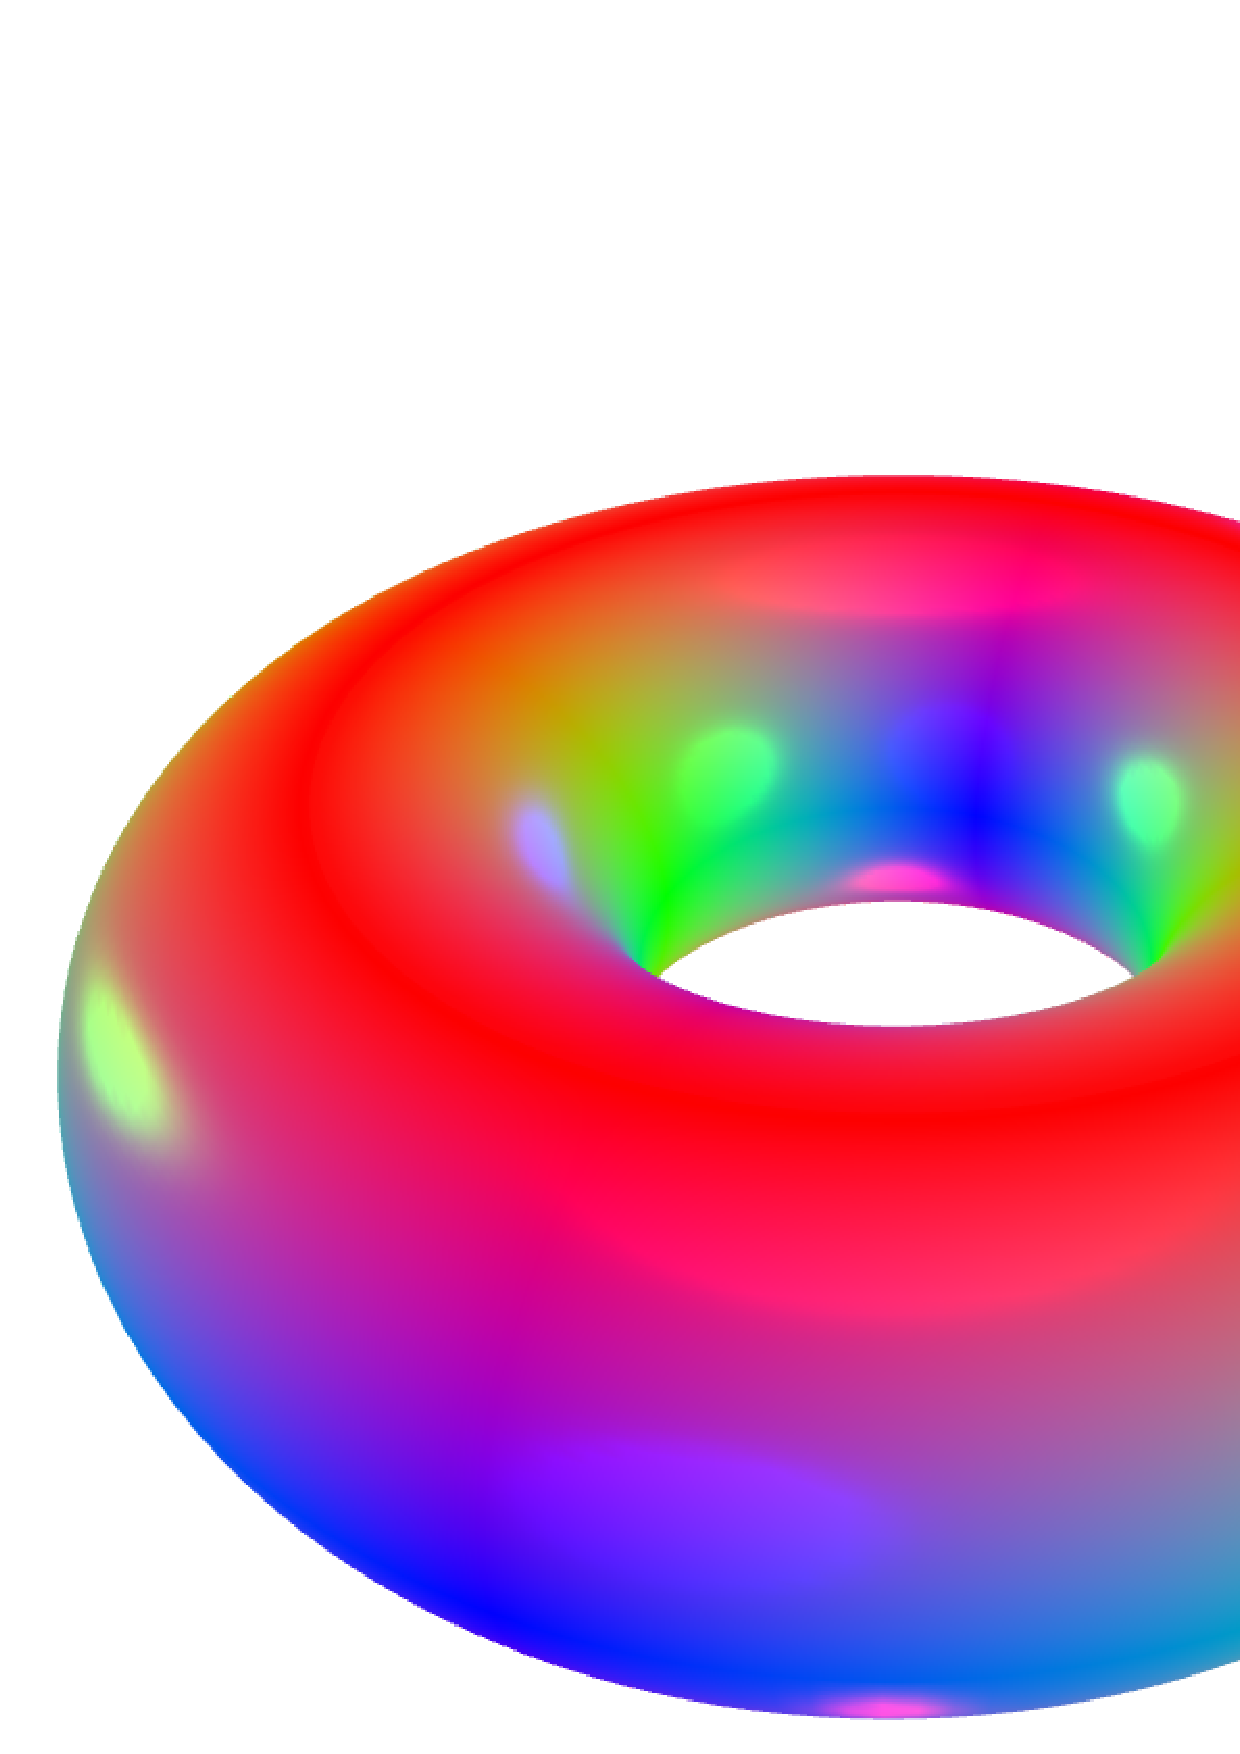
\includegraphics[height=0.8\textheight]{images/graphs/donut.png}
\end{frame}
\begin{frame}\frametitle{Sch\"one Graphen}
\includegraphics[height=0.8\textheight]{images/graphs/kleinsche_flasche.png}
\end{frame}
\begin{frame}\frametitle{Sch\"one Graphen}
\includegraphics[height=0.5\textheight]{images/graphs/limette.png}
\end{frame}
\begin{frame}\frametitle{Sch\"one Graphen}
\includegraphics[height=0.7\textheight]{images/graphs/schnecke.png}
\end{frame}
%%%%%%%%%%%%%%%%%%%%%%%%%%%%%%%%%%%%%%%%%%%%%%%%%%%%%%%%%%%%%%%%%%%%%%%%%%%%%%%%%%
\section{Arbeitsauftrag}
\begin{frame}\frametitle{Aufgabe 1}
\includegraphics[height=0.7\textheight]{images/graphs/x_divide_y.png}
\end{frame}
%%%%%%%%%%%%%%%%%%%%%%%%%%%%%%%%%%%%%%%%%%%%%%%%%%%%%%%%%%%%%%%%%%%%%%%%%%%%%%%%%%
\begin{frame}\frametitle{Aufgabe 2}
 \includegraphics[height=0.7\textheight]{images/graphs/sin_cos.png}
\end{frame}
%%%%%%%%%%%%%%%%%%%%%%%%%%%%%%%%%%%%%%%%%%%%%%%%%%%%%%%%%%%%%%%%%%%%%%%%%%%%%%%%%%
\begin{frame}\frametitle{Aufgabe 3}
  \includegraphics[height=0.7\textheight]{images/graphs/x_mod_y.png}
\end{frame}
%%%%%%%%%%%%%%%%%%%%%%%%%%%%%%%%%%%%%%%%%%%%%%%%%%%%%%%%%%%%%%%%%%%%%%%%%%%%%%%%%%
\begin{frame}\frametitle{Bonusaufgabe}
  \includegraphics[height=0.7\textheight]{images/graphs/sphere.png}
\end{frame}
%%%%%%%%%%%%%%%%%%%%%%%%%%%%%%%%%%%%%%%%%%%%%%%%%%%%%%%%%%%%%%%%%%%%%%%%%%%%%%%%%%


\end{document}

